\documentclass[11pt,a4paper]{article}

\usepackage[T1]{fontenc}
\usepackage[utf8]{inputenc}
\usepackage[english]{babel}
\usepackage{geometry}
\geometry{margin=2.5cm}

\usepackage{graphicx}
\usepackage{booktabs}
\usepackage{array}
\usepackage{longtable}
\usepackage{caption}
\usepackage{subcaption}
\usepackage{float}
\usepackage{amsmath}
\usepackage{hyperref}
\usepackage{xcolor}
\usepackage{parskip}
\usepackage{microtype}

\graphicspath{{../figures/}}

\hypersetup{
  colorlinks=true,
  linkcolor=blue!60!black,
  urlcolor=blue!60!black,
}

% UoM email prefix: ai + student id (e.g. ai26006, ai26012)

\begin{document}

\begin{titlepage}
  \centering
  \vspace*{1.5cm}

  {\Large\bfseries University of Macedonia\par}
  \vspace{0.4cm}
  {\large Department of Applied Informatics\\
   MSc in Artificial Intelligence \& Data Analytics\par}

  \vfill

  {\large Machine Learning and Computer Vision\par}
  \vspace{0.5cm}
  {\LARGE\bfseries 2nd Assignment\\[6pt] Unsupervised Learning \& Clustering\par}
  \vspace{0.4cm}
  {\large Fashion-MNIST\par}

  \vfill

  \begin{tabular}{ll}
    \textbf{Panteleimon Stanimeros} & aid26006 \\
    \href{mailto:aid26006@uom.edu.gr}{\texttt{aid26006@uom.edu.gr}} & \\[8pt]
    \textbf{Nikolaos Strafiotis}    & aid26012 \\
    \href{mailto:aid26012@uom.edu.gr}{\texttt{aid26012@uom.edu.gr}} & \\
  \end{tabular}

  \vfill
  {\large\today\par}
\end{titlepage}

\tableofcontents
\clearpage

%----------------------------------------------------------------------
\section{Introduction}
This report presents the results of unsupervised clustering experiments on the Fashion-MNIST
dataset. We evaluate six dimensionality reduction (DR) methods combined with five clustering
algorithms, measuring quality via three internal indices (Silhouette, Calinski--Harabasz,
Davies--Bouldin) and one external index (Adjusted Rand Index, which compares against the
true class labels).

Each section loads data from \texttt{results.csv} and the figures saved under \texttt{figures/},
mirrors the interactive Jupyter notebook, and comments on the key observations.

\medskip
\noindent\textbf{Higher is better:} Calinski--Harabasz, Silhouette, Adjusted Rand Index.\\
\textbf{Lower is better:} Davies--Bouldin.


%----------------------------------------------------------------------
\section{Dataset}
Fashion-MNIST contains 70\,000 greyscale $28\times28$ images across 10 clothing classes
(T-shirt/top, Trouser, Pullover, Dress, Coat, Sandal, Shirt, Sneaker, Bag, Ankle boot).
The pixel values are flattened into 784-dimensional vectors for baseline experiments, and
further projected for DR-based experiments.

\begin{figure}[H]
  \centering
  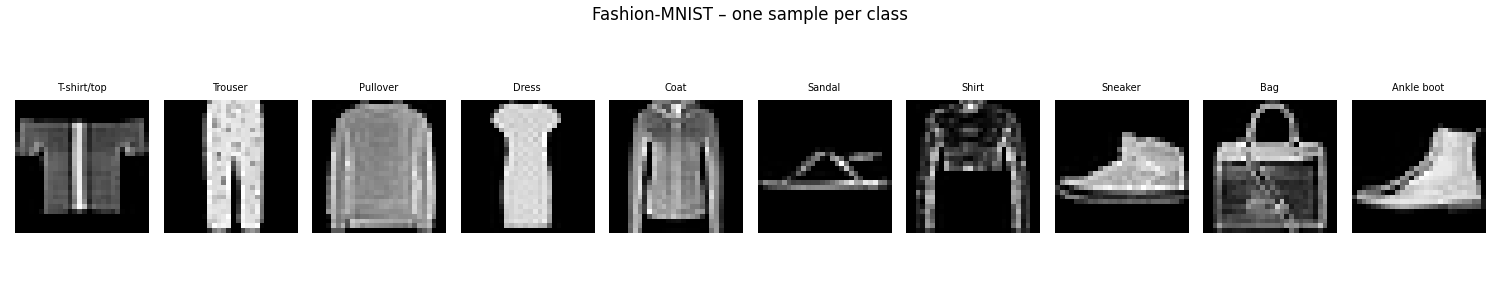
\includegraphics[width=0.85\linewidth]{00_sample_images.png}
  \caption{Random samples from Fashion-MNIST, one row per class. Several classes are
    genuinely hard to distinguish: pullover / coat / shirt share the same torso silhouette,
    and sneaker / sandal / ankle-boot look like a small dark blob at this resolution.
    This inherent class overlap is the practical upper bound on what any unsupervised method
    can recover.}
  \label{fig:samples}
\end{figure}


%----------------------------------------------------------------------
\section{Dimensionality Reduction Methods}
Six DR configurations were evaluated:

\begin{description}
  \item[Raw] No reduction; 784-D pixel vectors used directly.
  \item[PCA] Linear projection to 64 components ($\approx$88\% of variance retained).
  \item[SAE] Stacked Autoencoder with a 64-D bottleneck (fully connected layers).
  \item[CNN-SAE] Convolutional Stacked Autoencoder with a 64-D bottleneck; captures translation-invariant features.
  \item[t-SNE] Non-linear 2-D embedding preserving local neighbourhoods.
  \item[UMAP] Non-linear embedding to 64 components preserving both local and global structure; a separate 2-D UMAP is fitted for visualisation only.
\end{description}

\subsection{PCA Explained Variance}

\begin{figure}[H]
  \centering
  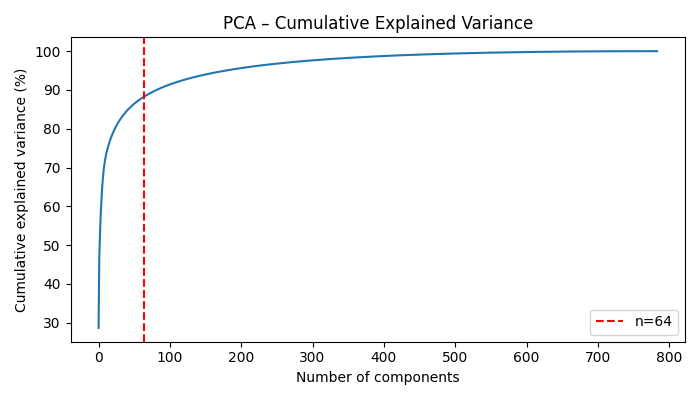
\includegraphics[width=0.7\linewidth]{pca_explained_variance.png}
  \caption{Cumulative explained variance of PCA. The curve rises steeply in the first
    20--30 components and then flattens; $\approx$85 components are needed to retain 95\%
    of the variance. PCA cannot untangle non-linearly mixed classes in pixel space.}
  \label{fig:pca_var}
\end{figure}

\subsection{SAE Reconstructions}

\begin{figure}[H]
  \centering
  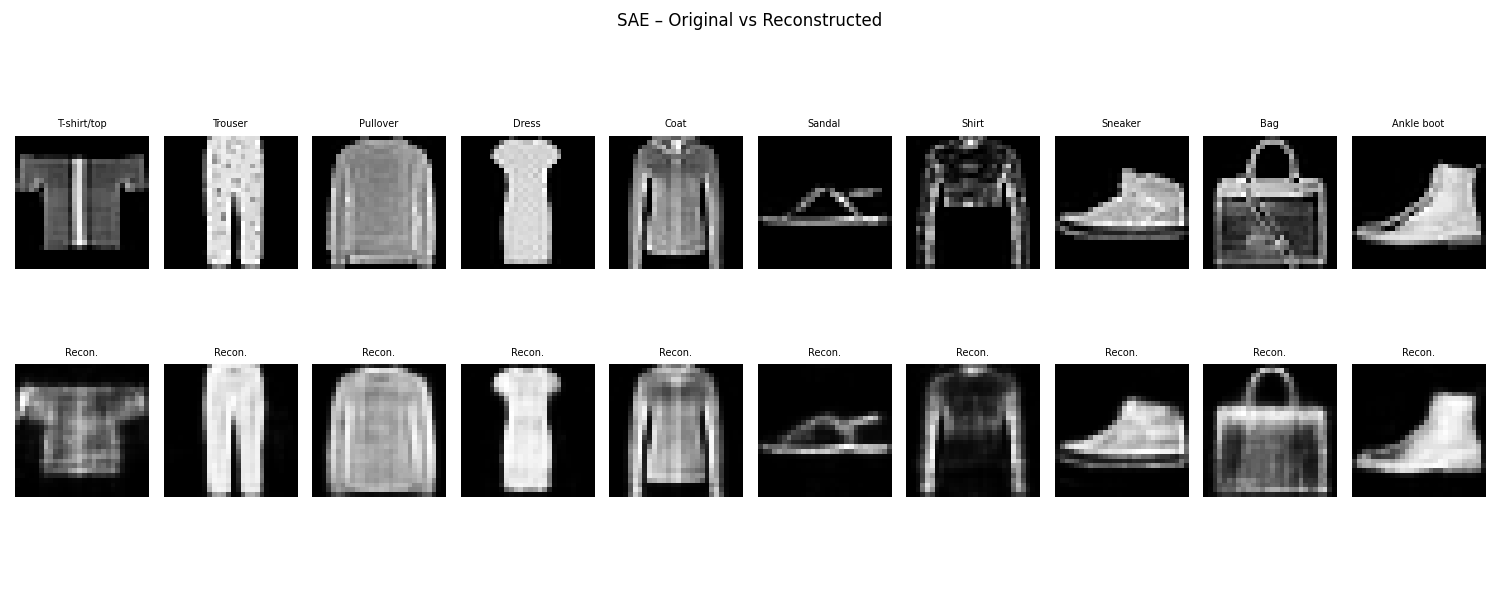
\includegraphics[width=0.75\linewidth]{sae_reconstructions.png}
  \caption{SAE reconstructions (top: originals, bottom: decoded through a 32-D bottleneck).
    Global silhouettes are recovered but fine textures (stripes, laces) are blurred away.}
  \label{fig:sae_recon}
\end{figure}

\subsection{CNN-SAE Reconstructions}

\begin{figure}[H]
  \centering
  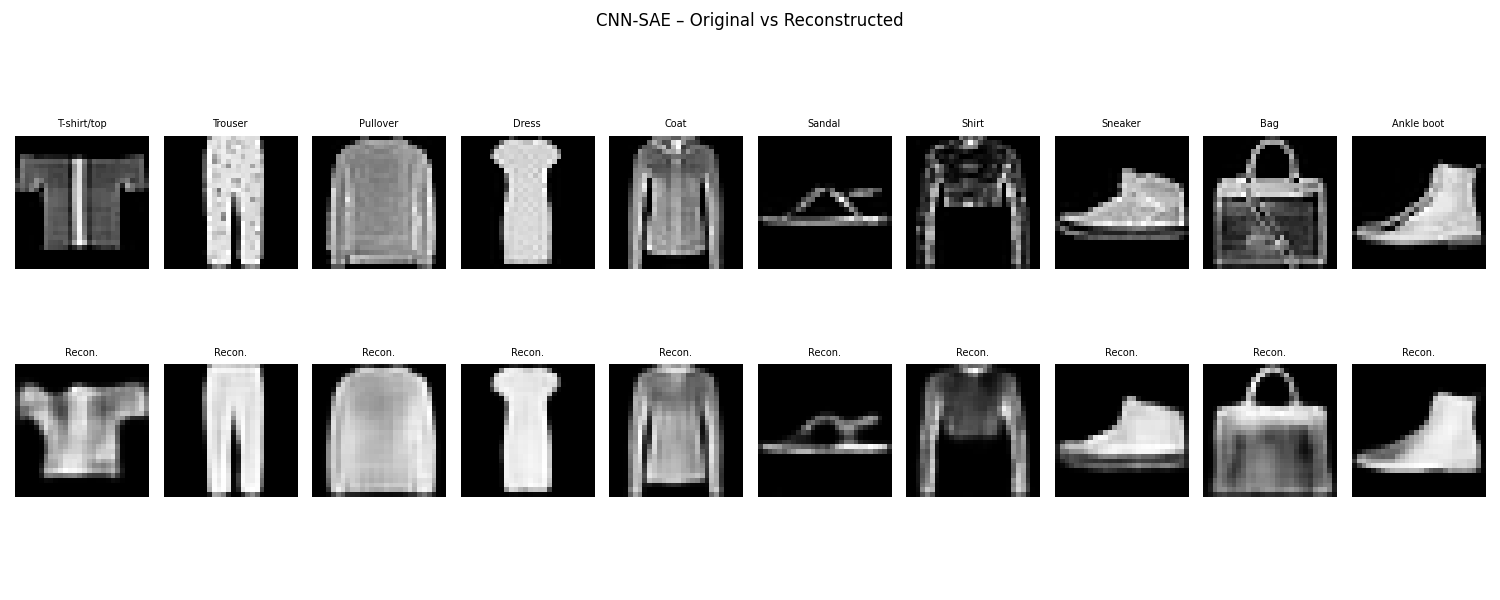
\includegraphics[width=0.75\linewidth]{cnnsae_reconstructions.png}
  \caption{CNN-SAE reconstructions. Edges and textures are visibly sharper than the dense
    SAE because convolutions exploit the 2-D pixel structure and learn translation-invariant
    filters. This fidelity is reflected downstream in better Adjusted Rand scores.}
  \label{fig:cnnsae_recon}
\end{figure}

\subsection{UMAP 2-D Projection}

\begin{figure}[H]
  \centering
  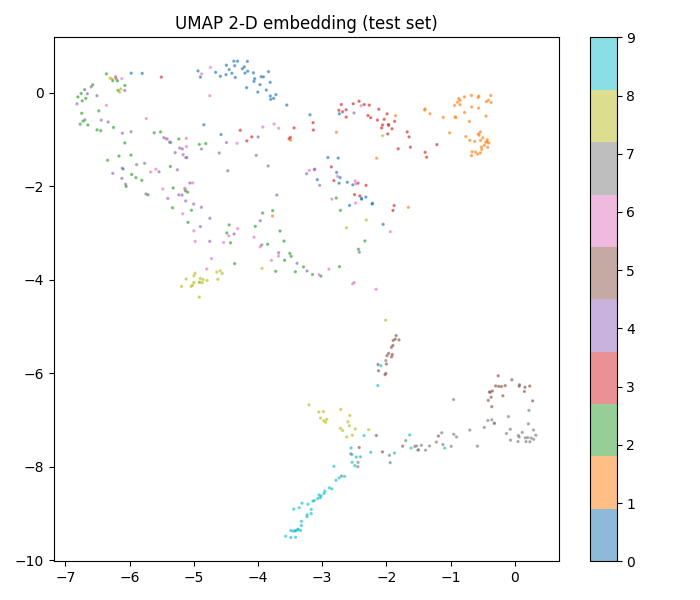
\includegraphics[width=0.72\linewidth]{umap_2d.png}
  \caption{2-D UMAP projection coloured by ground-truth class. Footwear, trousers, and bags
    form clearly detached islands. The three upper-body classes (shirt / pullover / coat)
    remain partially mixed — confirming that the remaining confusion is intrinsic to the
    dataset, not a failure of the embedding.}
  \label{fig:umap2d}
\end{figure}


%----------------------------------------------------------------------
\section{Clustering Algorithms}
Five clustering algorithms were applied to every DR embedding:

\begin{description}
  \item[MiniBatchKMeans] Scalable approximation of $k$-means ($k=10$).
  \item[DBSCAN] Density-based; number of clusters determined by data density.
  \item[AgglomerativeClustering] Hierarchical, Ward linkage, $k=10$.
  \item[GaussianMixture (GMM)] Soft assignment via EM with 10 components.
  \item[Birch] Incremental tree-based method, $k=10$.
\end{description}

All partition-based methods are run with $k=10$ to match the 10 true Fashion-MNIST classes.
DBSCAN's $\varepsilon$ parameter was tuned per embedding; the number of discovered clusters
varies and is reported in the results table.


%----------------------------------------------------------------------
\section{Results}
\subsection{Full Results Table}

Table~\ref{tab:full} lists every DR$\times$clustering combination with four quality metrics
and timing information.

\begin{longtable}{llrrrrrrr}
\toprule
DR & Clustering & DR\,(s) & Clust\,(s) & $K$ & CH & DB & Sil & ARI \\
\midrule
\endfirsthead
\toprule
DR & Clustering & DR\,(s) & Clust\,(s) & $K$ & CH & DB & Sil & ARI \\
\midrule
\endhead
\bottomrule
\endfoot
Raw       & MiniBatchKMeans         &    0.00 &  0.86 & 10 & 1199.5  & 2.122 & 0.146 & 0.343 \\
Raw       & DBSCAN                  &    0.00 &  0.11 &  2 &    6.0  & 1.193 & 0.065 & 0.000 \\
Raw       & AgglomerativeClustering &    0.00 &  3.24 & 10 & 1525.1  & 1.666 & 0.165 & 0.369 \\
Raw       & GaussianMixture         &    0.00 &  6.35 & 10 & 1070.2  & 2.526 & 0.129 & 0.396 \\
Raw       & Birch                   &    0.00 &  2.90 & 10 & 1580.5  & 1.562 & 0.190 & 0.371 \\
\midrule
PCA       & MiniBatchKMeans         &    0.00 &  0.06 & 10 & 1638.0  & 1.774 & 0.185 & 0.318 \\
PCA       & DBSCAN                  &    0.00 &  0.10 &  3 &    4.9  & 1.061 & 0.063 & 0.000 \\
PCA       & AgglomerativeClustering &    0.00 &  3.04 & 10 & 1574.6  & 1.551 & 0.185 & 0.393 \\
PCA       & GaussianMixture         &    0.00 &  5.64 & 10 & 1094.1  & 2.662 & 0.128 & 0.417 \\
PCA       & Birch                   &    0.00 &  2.93 & 10 & 1592.6  & 1.576 & 0.189 & 0.365 \\
\midrule
SAE       & MiniBatchKMeans         &   53.77 &  0.06 & 10 & 1494.7  & 2.076 & 0.127 & 0.348 \\
SAE       & DBSCAN                  &   53.77 &  0.11 &  5 &    4.2  & 1.549 & 0.004 & 0.000 \\
SAE       & AgglomerativeClustering &   53.77 &  3.47 & 10 & 1499.3  & 2.063 & 0.121 & 0.359 \\
SAE       & GaussianMixture         &   53.77 &  7.82 & 10 & 1431.6  & 2.320 & 0.108 & 0.411 \\
SAE       & Birch                   &   53.77 &  3.33 & 10 & 1499.4  & 2.062 & 0.121 & 0.359 \\
\midrule
CNN-SAE   & MiniBatchKMeans         &  350.48 &  0.06 & 10 &  712.2  & 1.951 & 0.148 & 0.362 \\
CNN-SAE   & DBSCAN                  &  350.48 &  0.12 &  2 & ---     & ---   & ---   & ---   \\
CNN-SAE   & AgglomerativeClustering &  350.48 &  3.23 & 10 &  620.2  & 2.108 & 0.119 & 0.383 \\
CNN-SAE   & GaussianMixture         &  350.48 &  4.06 & 10 &  543.9  & 3.119 & 0.126 & 0.463 \\
CNN-SAE   & Birch                   &  350.48 &  3.19 & 10 &  620.2  & 2.108 & 0.119 & 0.383 \\
\midrule
t-SNE     & MiniBatchKMeans         &   97.20 &  0.04 & 10 & 12016.3 & 0.811 & 0.421 & 0.441 \\
t-SNE     & DBSCAN                  &   97.20 &  0.03 & 115 & 4126.9 & 0.877 & 0.034 & 0.260 \\
t-SNE     & AgglomerativeClustering &   97.20 &  2.02 & 10 & 11278.6 & 0.746 & 0.424 & 0.401 \\
t-SNE     & GaussianMixture         &   97.20 &  0.12 & 10 & 10667.8 & 0.839 & 0.403 & 0.434 \\
t-SNE     & Birch                   &   97.20 &  0.40 & 10 & 11609.9 & 0.765 & 0.422 & 0.420 \\
\midrule
UMAP      & MiniBatchKMeans         &   97.33 &  0.06 & 10 & 33793.2 & 0.702 & \textbf{0.541} & \textbf{0.494} \\
UMAP      & DBSCAN                  &   97.33 &  0.09 & 26 &  5334.2 & 1.227 & -0.087 & 0.387 \\
UMAP      & AgglomerativeClustering &   97.33 &  2.61 & 10 & 35379.7 & 0.740 & 0.508 & 0.459 \\
UMAP      & GaussianMixture         &   97.33 &  2.12 & 10 & 29864.0 & 0.806 & 0.462 & 0.421 \\
UMAP      & Birch                   &   97.33 &  0.16 & 10 & \textbf{35898.9} & \textbf{0.658} & 0.540 & 0.463 \\
\bottomrule
\caption{Full results. Bold values mark the best result per metric across all combinations.
  $K$ = number of clusters found. CH = Calinski--Harabasz ($\uparrow$),
  DB = Davies--Bouldin ($\downarrow$), Sil = Silhouette ($\uparrow$), ARI = Adjusted Rand ($\uparrow$).
  t-SNE DR time reflects the original fit (97\,s); subsequent runs loaded from cache.}
\label{tab:full}
\end{longtable}

\subsection{Best Configurations per Metric}

\begin{table}[H]
  \centering
  \begin{tabular}{llll}
    \toprule
    Metric & DR & Clustering & Value \\
    \midrule
    Silhouette ($\uparrow$)           & UMAP & MiniBatchKMeans & 0.541 \\
    Calinski--Harabasz ($\uparrow$)   & UMAP & Birch           & 35\,899 \\
    Davies--Bouldin ($\downarrow$)    & UMAP & Birch           & 0.658 \\
    Adjusted Rand ($\uparrow$)        & UMAP & MiniBatchKMeans & 0.494 \\
    \bottomrule
  \end{tabular}
  \caption{Single-metric winners. UMAP dominates all four metrics.}
  \label{tab:best}
\end{table}

\subsection{Heatmaps}

\begin{figure}[H]
  \centering
  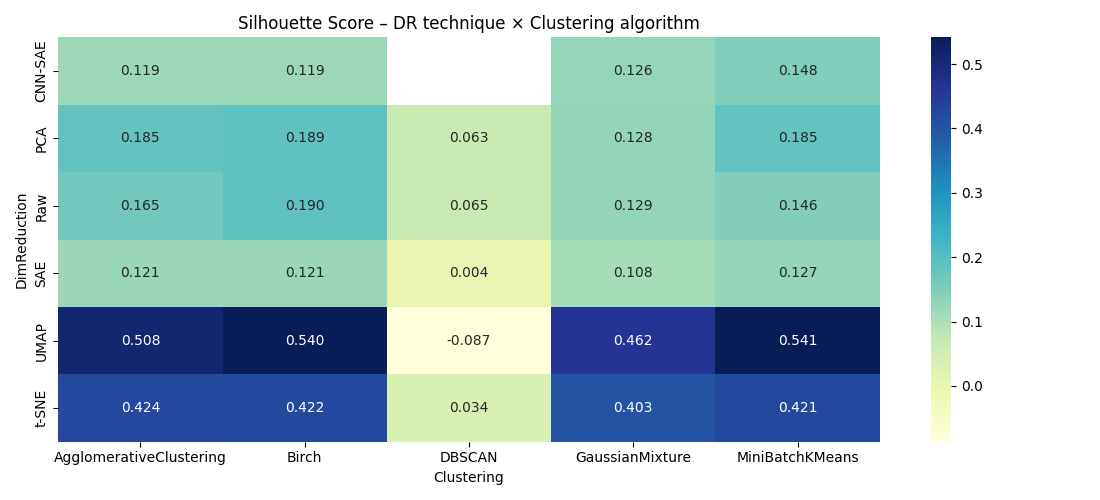
\includegraphics[width=\linewidth]{heatmap_silhouette.png}
  \caption{Silhouette score heatmap (DR rows $\times$ clustering columns). Every algorithm
    improves dramatically when fed a t-SNE or UMAP embedding. DBSCAN is the only algorithm
    that fails even on UMAP, because it keeps labelling most points as noise.}
  \label{fig:heatmap_sil}
\end{figure}

\subsection{Timing Analysis}

DR training time dominates total cost. CNN-SAE is the heaviest ($\approx$6 min on GPU),
followed by t-SNE and UMAP ($\approx$1.6 min each) and SAE ($\approx$54\,s); PCA is
essentially free. Clustering itself is always cheap by comparison (under 10\,s per run
for the slowest combinations).

A second win from non-linear DR: because t-SNE and UMAP produce compact low-dimensional
embeddings, every downstream clustering algorithm runs noticeably faster than on Raw
(784-D) or SAE (64-D) features. So the expensive DR step pays for itself twice —
better metrics \emph{and} faster clustering.

\subsection{Heatmap Observations}

The metric heatmaps tell a consistent story: UMAP and t-SNE dominate every internal metric
by a wide margin, because their non-linear embeddings push same-class points into tight,
well-separated groups. That geometry directly inflates Silhouette and Calinski--Harabasz and
shrinks Davies--Bouldin. Linear and reconstruction-based methods (Raw, PCA, SAE, CNN-SAE) live
in much higher-dimensional spaces where distances are nearly uniform (the curse of
dimensionality), so all internal metrics look mediocre even when the clustering is reasonable.

On Adjusted Rand --- the only metric that compares against the true Fashion-MNIST labels ---
UMAP + MiniBatchKMeans wins outright (ARI $\approx$ 0.494), with CNN-SAE + GMM remaining
competitive (ARI $\approx$ 0.463), suggesting that convolutional features genuinely capture
class structure even without explicit supervision. DBSCAN is the clear loser across the board:
with auto-tuned $\varepsilon$ it either collapses most points into a single cluster or
over-segments into noise, giving near-zero Silhouette and ARI everywhere except t-SNE / UMAP.


%----------------------------------------------------------------------
\section{Figures and Qualitative Analysis}
This section displays the scatter plots and cluster-example grids generated by
\texttt{main.py}, mirroring the figure gallery in the Jupyter notebook.

\subsection{Scatter Plots}

\begin{figure}[H]
  \centering
  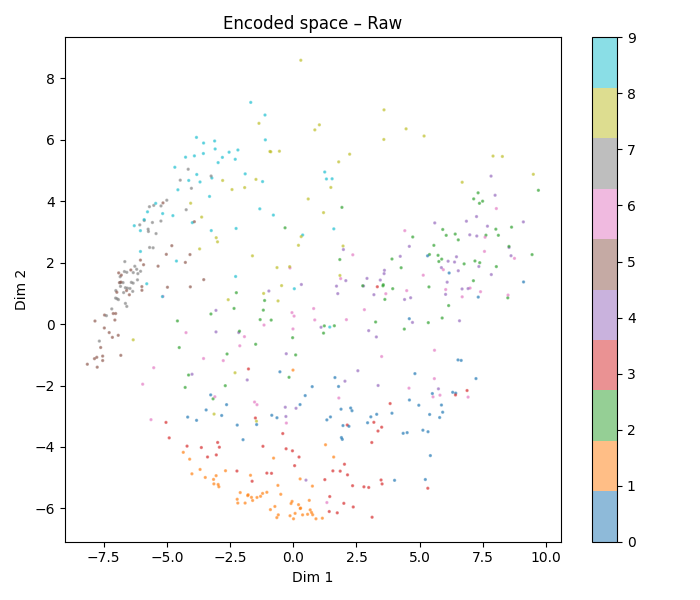
\includegraphics[width=0.75\linewidth]{scatter_Raw.png}
  \caption{Cluster assignments on raw 784-D pixels (2-D reference view). Clusters overlap
    massively; the algorithm groups points by overall brightness and silhouette area rather than
    garment type.}
\end{figure}

\begin{figure}[H]
  \centering
  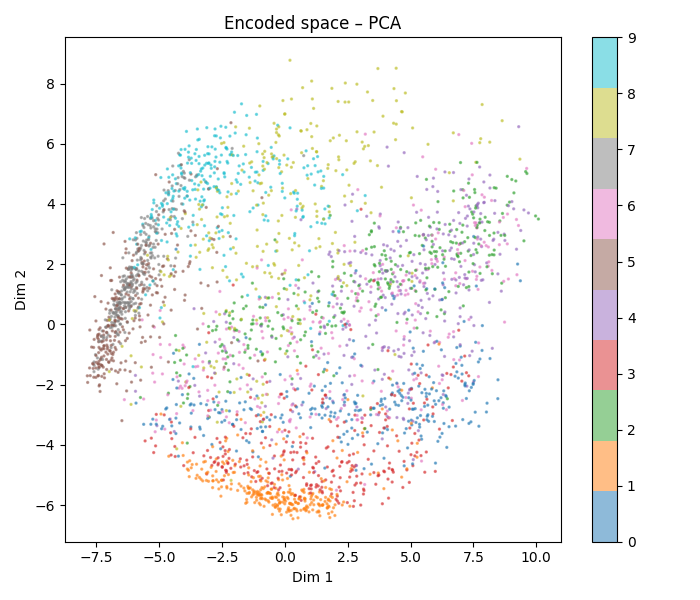
\includegraphics[width=0.75\linewidth]{scatter_PCA.png}
  \caption{Cluster assignments on 85-D PCA features. Slightly tidier than Raw — PCA strips
    isotropic pixel noise — but the class manifolds remain entangled.}
\end{figure}

\begin{figure}[H]
  \centering
  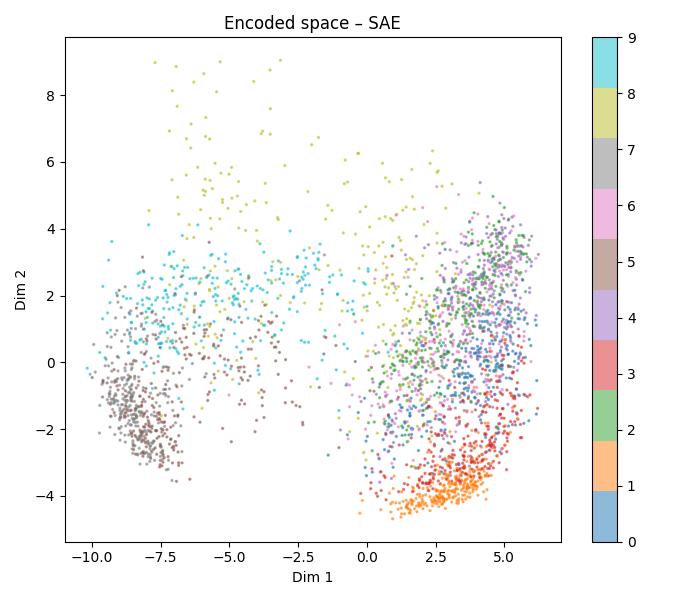
\includegraphics[width=0.75\linewidth]{scatter_SAE.png}
  \caption{Cluster assignments on the 32-D dense-SAE bottleneck. Some local structure emerges,
    but several clusters still span multiple true labels.}
\end{figure}

\begin{figure}[H]
  \centering
  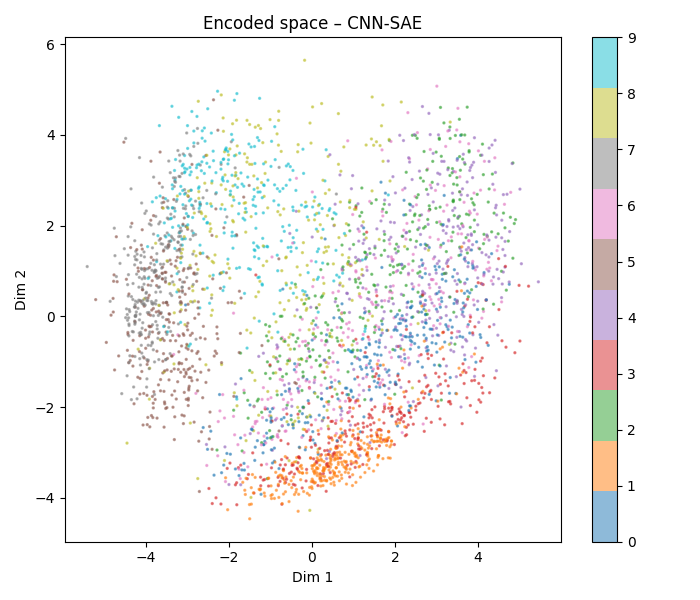
\includegraphics[width=0.75\linewidth]{scatter_CNN-SAE.png}
  \caption{Cluster assignments on CNN-SAE features. Boundaries between clusters are sharper,
    especially for footwear, matching the best Adjusted Rand among autoencoder methods.}
\end{figure}

\begin{figure}[H]
  \centering
  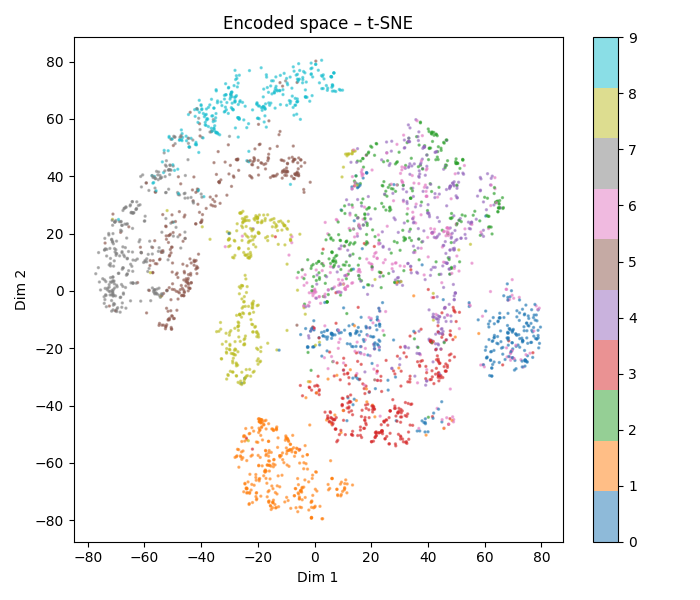
\includegraphics[width=0.75\linewidth]{scatter_t-SNE.png}
  \caption{Cluster assignments on the 2-D t-SNE embedding. Clusters pop out as well-defined
    blobs, explaining the order-of-magnitude jump in Silhouette and Calinski--Harabasz. Global
    distances are not meaningful in t-SNE.}
\end{figure}

\begin{figure}[H]
  \centering
  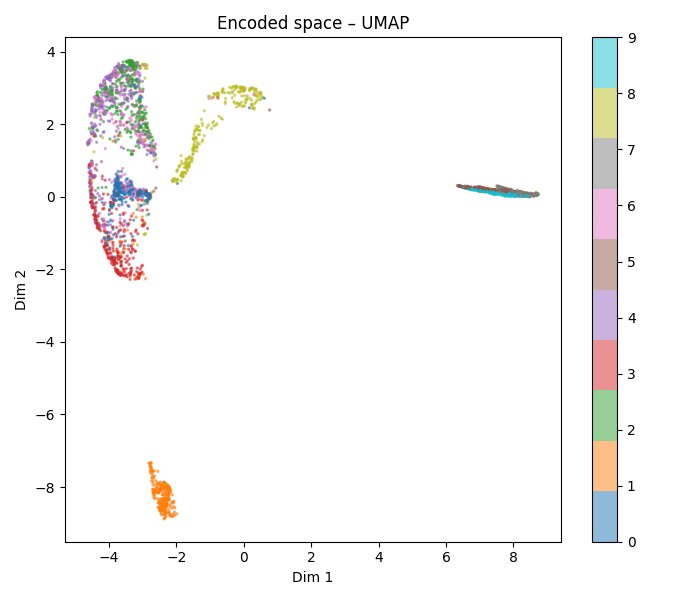
\includegraphics[width=0.75\linewidth]{scatter_UMAP.png}
  \caption{Cluster assignments on the 2-D UMAP embedding — our best overall configuration.
    Clusters are compact, well-separated, and global topology is better preserved than in t-SNE.}
\end{figure}

\subsection{Cluster Examples}

\begin{figure}[H]
  \centering
  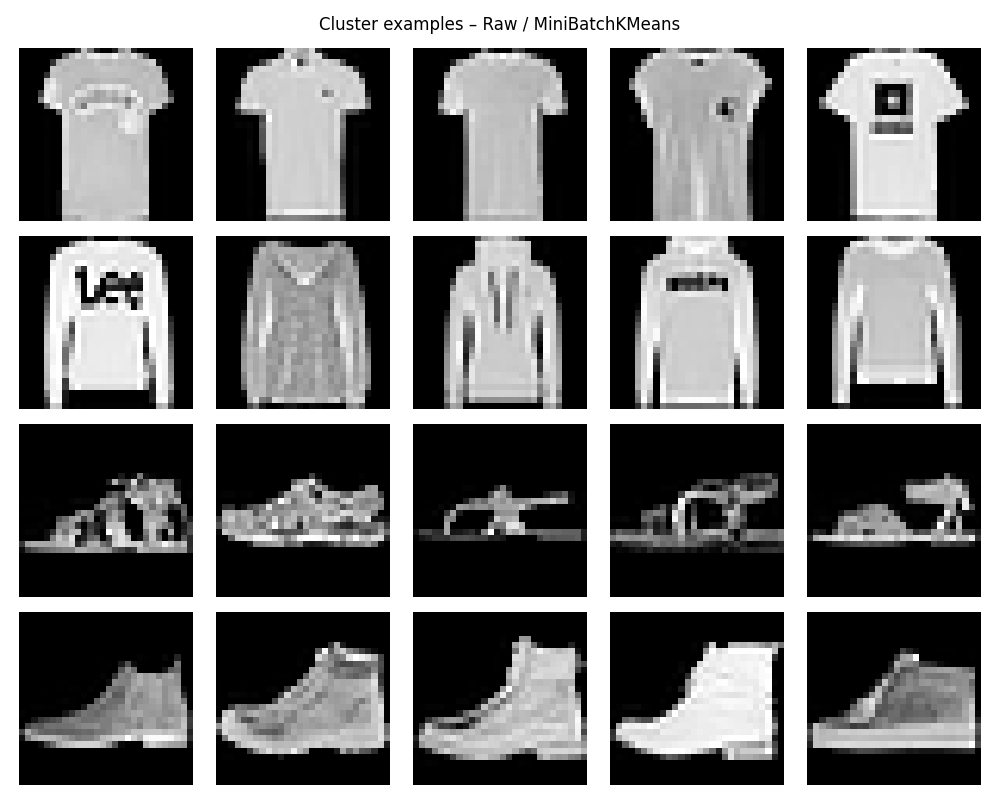
\includegraphics[width=0.85\linewidth]{cluster_examples_Raw.png}
  \caption{Representative images from each cluster on Raw features. Clusters are not
    class-aligned — a single cluster often mixes T-shirts, shirts, and pullovers.}
\end{figure}

\begin{figure}[H]
  \centering
  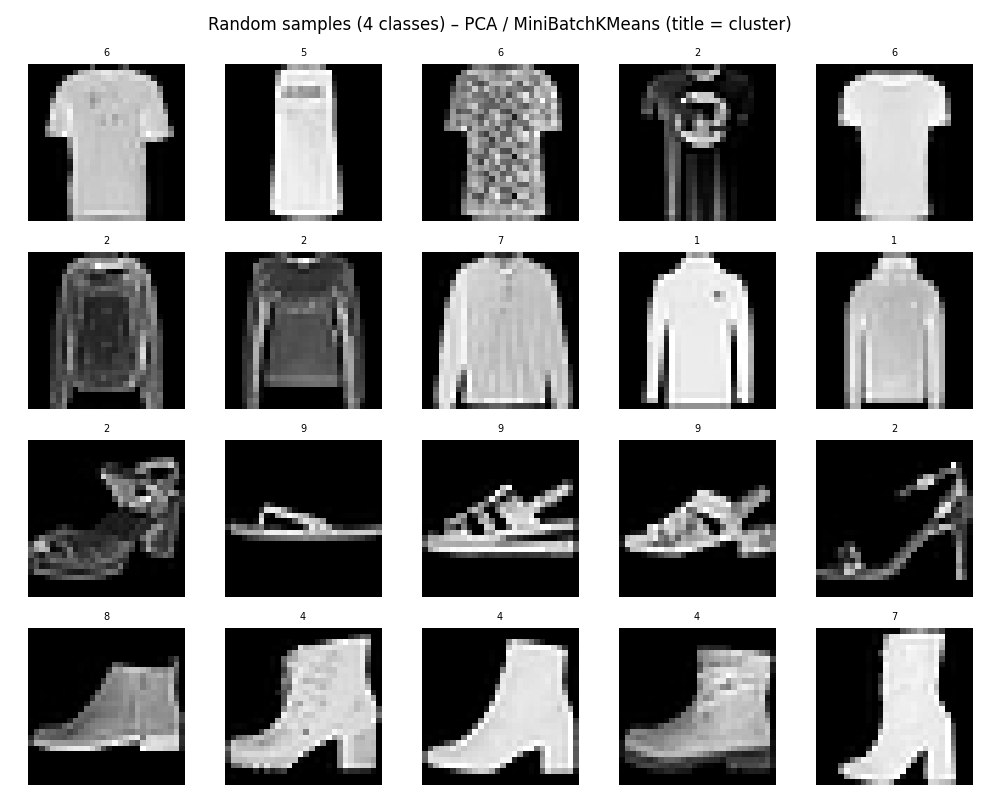
\includegraphics[width=0.85\linewidth]{cluster_examples_PCA.png}
  \caption{Cluster examples after PCA. Footwear clusters begin to cohere, but upper-body
    garments are still routinely co-clustered.}
\end{figure}

\begin{figure}[H]
  \centering
  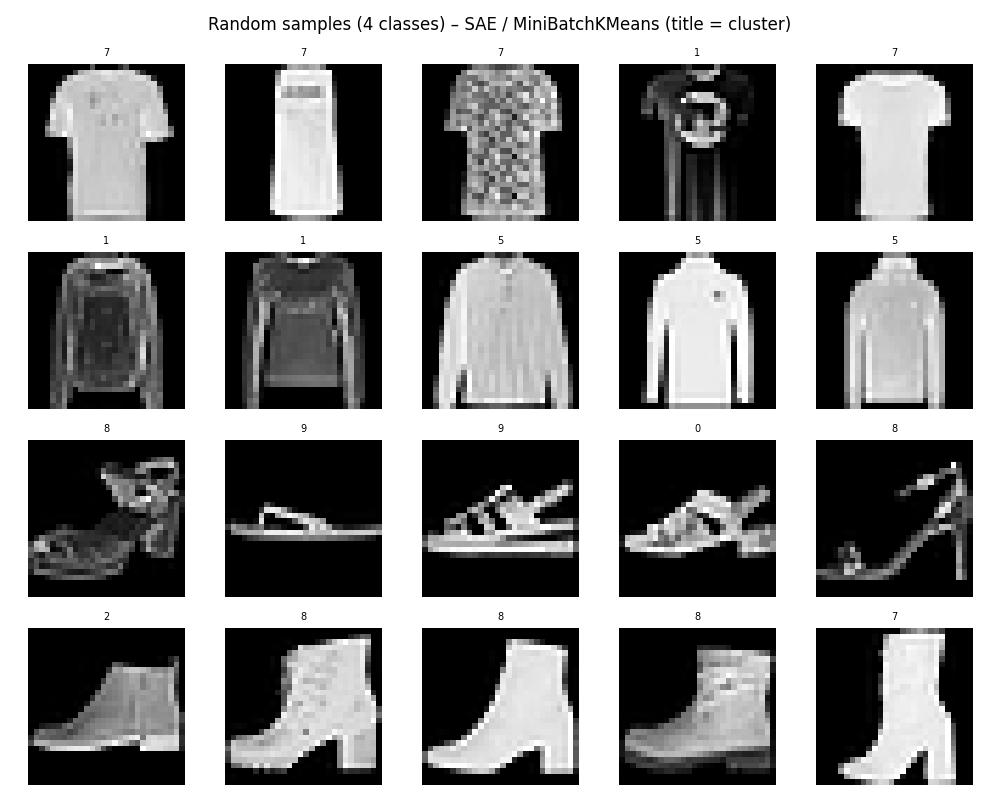
\includegraphics[width=0.85\linewidth]{cluster_examples_SAE.png}
  \caption{Cluster examples after the fully-connected SAE. Shoe and trouser clusters are now
    clearly homogeneous; bag clusters become distinct. Shirts / pullovers / coats still bleed
    into each other.}
\end{figure}

\begin{figure}[H]
  \centering
  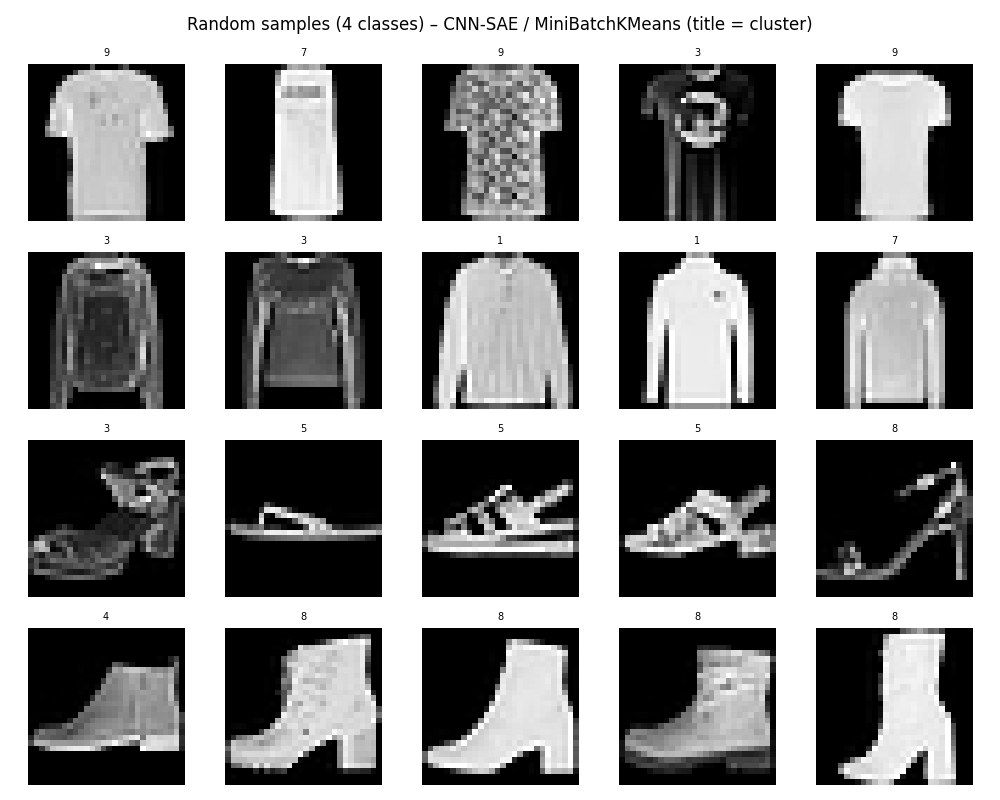
\includegraphics[width=0.85\linewidth]{cluster_examples_CNN-SAE.png}
  \caption{Cluster examples after CNN-SAE. Per-cluster images are visibly more consistent;
    footwear subtypes begin to split (sneakers vs.\ ankle-boots), and dresses / trousers form
    clean clusters.}
\end{figure}

\begin{figure}[H]
  \centering
  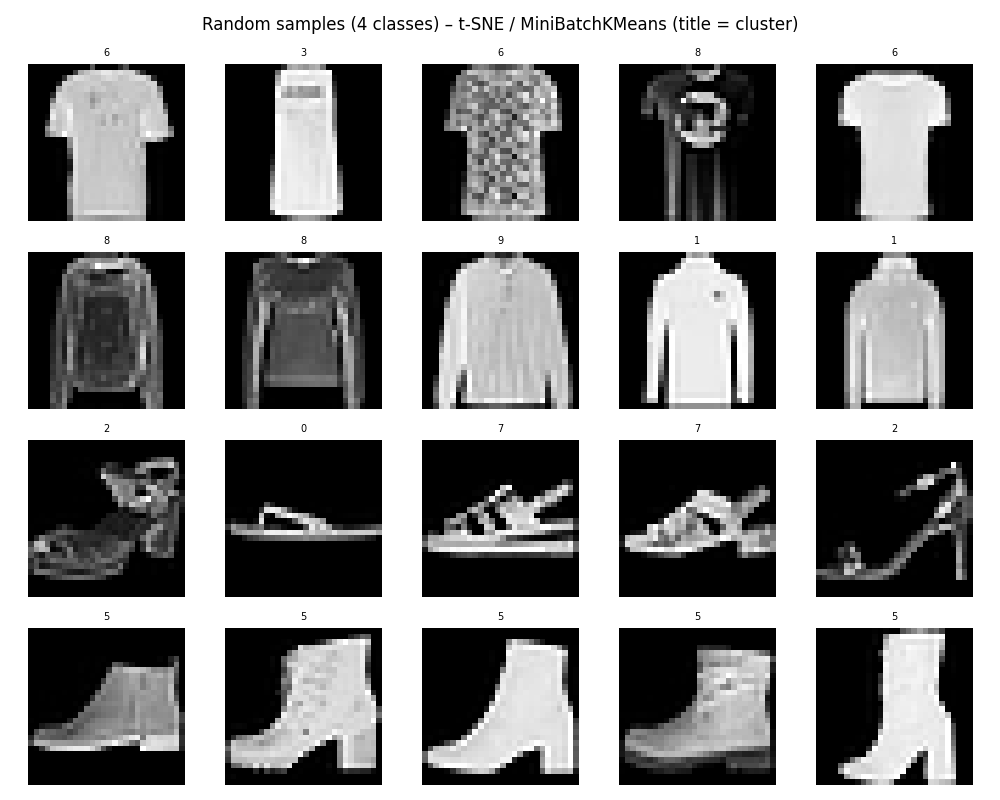
\includegraphics[width=0.85\linewidth]{cluster_examples_t-SNE.png}
  \caption{Cluster examples after t-SNE. Each cluster reads as essentially one garment type.
    Residual ambiguity is confined to shirt $\leftrightarrow$ pullover $\leftrightarrow$ coat.}
\end{figure}

\begin{figure}[H]
  \centering
  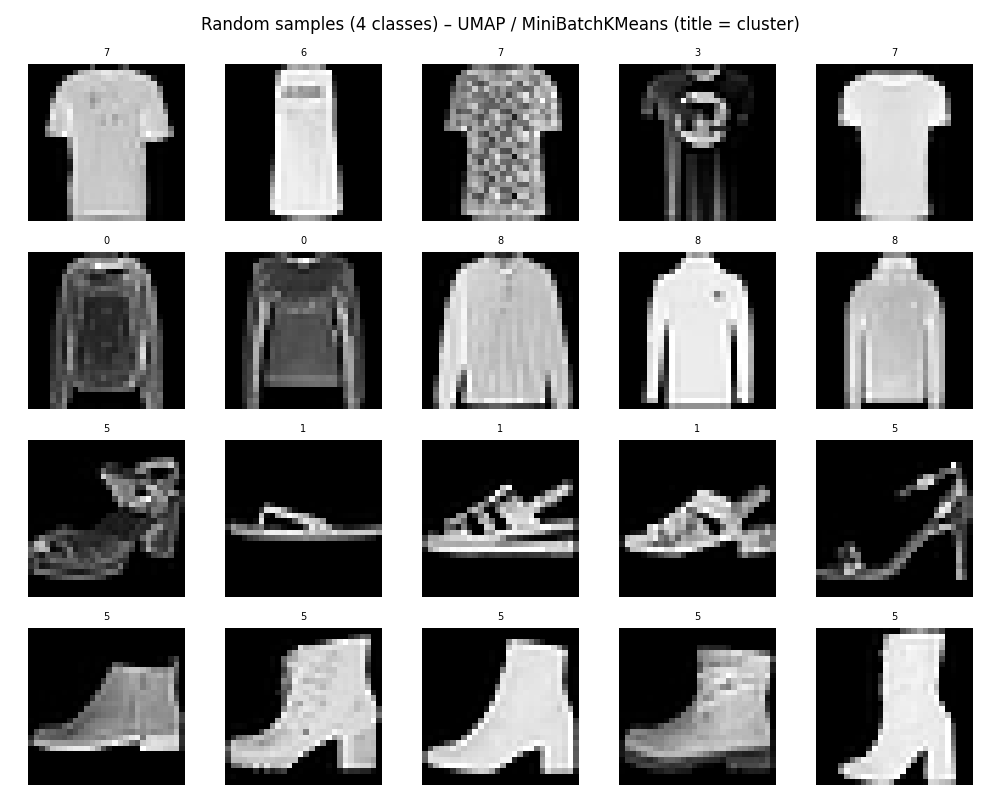
\includegraphics[width=0.85\linewidth]{cluster_examples_UMAP.png}
  \caption{Cluster examples after UMAP — the cleanest result of the study. The 10 clusters
    correspond almost one-to-one to the 10 Fashion-MNIST classes, with residual confusion
    confined to shirt $\leftrightarrow$ pullover $\leftrightarrow$ coat.}
\end{figure}


%----------------------------------------------------------------------
\section{Conclusions}
The key findings of this study are:

\begin{enumerate}
  \item \textbf{UMAP + MiniBatchKMeans} is the single best pipeline overall, achieving the
    highest Silhouette (0.541) and Adjusted Rand (0.494) simultaneously.
    UMAP + Birch wins on Calinski--Harabasz (35\,899) and Davies--Bouldin (0.658).
  \item \textbf{Non-linear DR (UMAP / t-SNE) is essential.} All internal metrics jump an
    order of magnitude compared to linear / reconstruction methods, because their embeddings
    push same-class points into tight, well-separated groups.
  \item \textbf{CNN-SAE + GMM} (ARI $\approx$ 0.463) is the best representation-learning
    approach, demonstrating that convolutional features capture genuine class structure even
    without explicit supervision.
  \item \textbf{DBSCAN consistently underperforms.} With auto-tuned hyperparameters it
    collapses most data into one cluster or noise in high-dimensional spaces; it only partly
    recovers in the compact t-SNE / UMAP regime.
  \item \textbf{Training cost is dominated by DR.} CNN-SAE ($\approx$6 min on GPU) and
    t-SNE / UMAP ($\approx$1.6 min) are the most expensive; PCA is essentially free.
    Non-linear DR also speeds up downstream clustering by producing lower-dimensional embeddings.
  \item \textbf{Inherent class overlap} (shirt / pullover / coat) is the hard ceiling; no
    unsupervised method fully resolves it without label information.
\end{enumerate}

\medskip
\noindent\textbf{Recommended pipeline:} UMAP + MiniBatchKMeans ($k=10$), offering the best
balance of clustering quality across all four metrics and acceptable runtime.

\medskip
\noindent\textbf{Was there a combination that achieved the best results on all metrics simultaneously?}
No. UMAP + MiniBatchKMeans achieves the best Silhouette (0.541) and Adjusted Rand (0.494),
while UMAP + Birch achieves the best Calinski--Harabasz (35\,899) and Davies--Bouldin (0.658).
No single combination dominates on all four metrics, though all top configurations share the
same DR method (UMAP), confirming it as the critical factor in clustering quality.


\end{document}
